\section{Questão 03}

\subsection{Item A}
O item A da questão três induz um teste da propriedade de comutatividade de uma operação de convolução. Assim, dois sinais foram definidos, e duas convoluções foram realizadas. A primeira foi realizada utilizando $(x, h)$ e a segunda $(h, x)$. Em seguida, utilizou-se o método \textit{stem} para a representação do resultado final dessas convoluções.

Na Figura \ref{fig:graph_17}, encontra-se a primeira convolução. 

\begin{figure}[!htb]
    \centering
    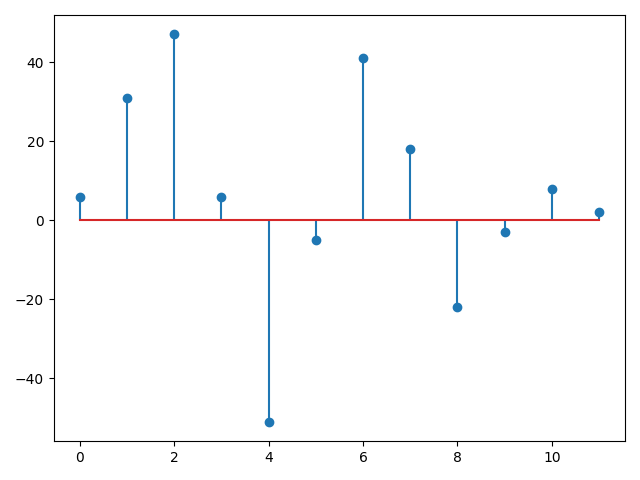
\includegraphics[width=\linewidth]{Imagens/fig17.png}
    \caption{Convolução de (x, h)}
    \label{fig:graph_17}
\end{figure}

Na Figura \ref{fig:graph_18}, encontra-se a convolução com a ordem dos argumentos alternada.

\begin{figure}[!htb]
    \centering
    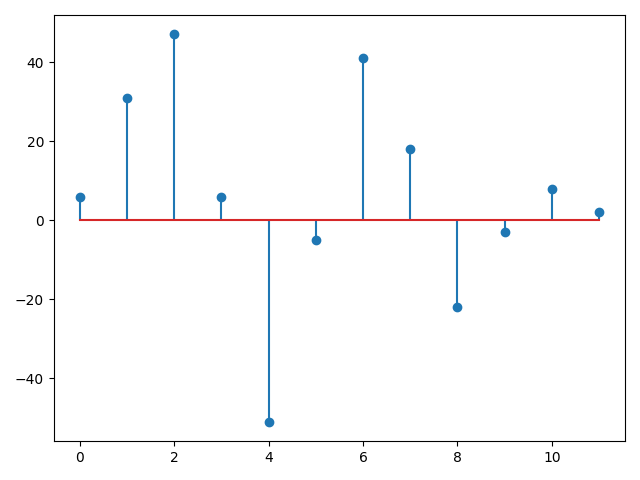
\includegraphics[width=\linewidth]{Imagens/fig18.png}
    \caption{Convolução de (h, x)}
    \label{fig:graph_18}
\end{figure}

Ao se comparar as Figuras \ref{fig:graph_17} e \ref{fig:graph_18}, conclui-se que a propriedade de comutatividade se fez presente na operação de convolução, uma vez que ambos resultados foram correspondentes.

\subsection{Item B}

Quando a convolução é realizada utilizando as funções \texttt{conv()} em \textit{Octave} ou \texttt{np.convolve()}
 em \textit{Python}, os índices temporais de cada sinal não são levados me conta ao se realizar as convoluções. Isso acaba gerando conflitos de resultado pois ao não se considerar os índices de cada vetor de valores, o resultado terá como índice inicial o $n = 0$. Porém, dependendo dos índices dos vetores iniciais, essa convolução pode ter que ser deslocada no eixo temporal para que demonstre o verdadeiro resultado esperado.

 Assim, criou-se um método que, diferente das funções convencionais acima que possuem como assinatura apenas os dois sinais de entrada, considera como argumentos 4 atributos: os dois vetores de sinais e os seus dois índices temporais. Como resultado final, obtém-se dois vetores: o resultado da convolução, obtida através das funções convencionais, e o vetor temporal. Dessa forma, o resultado dessa convolução será representado na posição temporal correta.

 \begin{figure}[!htb]
    \centering
    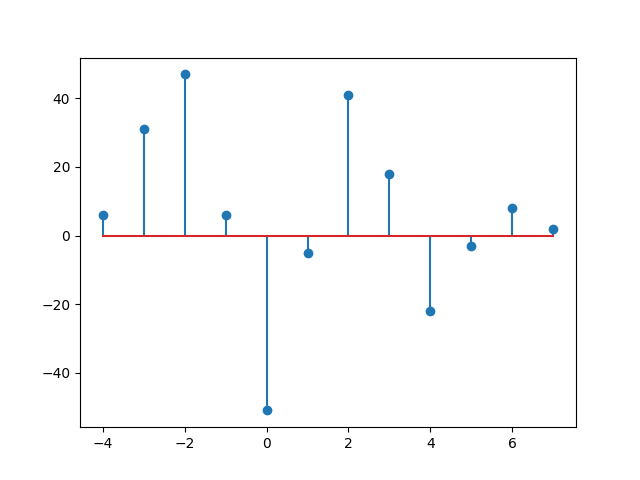
\includegraphics[width=\linewidth]{Imagens/fig19.png}
    \caption{Convolução de (h, x) com localização temporal}
    \label{fig:graph_19}
\end{figure}

 Na Figura \ref{fig:graph_19}, percebe-se que o resultado da convolução se mantém congruentes aos resultados obtidos anteriormente. Porém, ao se analisar o eixo temporal, verifica-se que o resultado se encontra deslocado para a esquerda. Esse deslocamento é explicado pelos vetores de índices temporais fornecidos ao método criado, que é capaz de atribuir um valor do resultado da convolução para o seu respectivo índice temporal. 

\subsection{Item C}
No item C, inicialmente, encontram-se duas funções senoidais com frequências distintas porém harmônicas. Esses sinais são somados para que se forme a função $x[n]$. 

O sinal $x[n]$ se encontra na Figura \ref{fig:graph_20}. 

\begin{figure}[!htb]
    \centering
    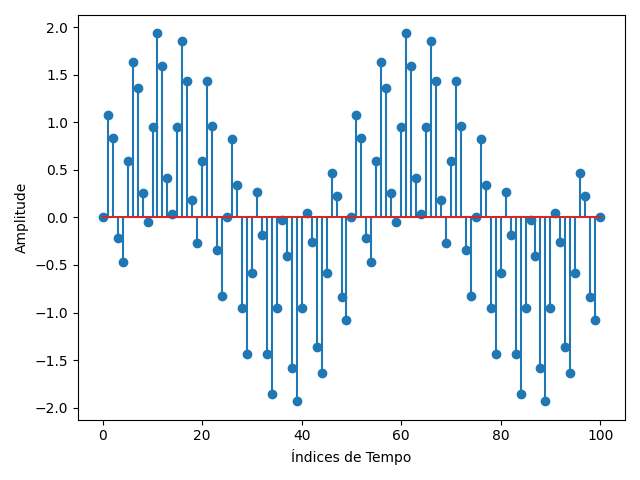
\includegraphics[width=\linewidth]{Imagens/fig20.png}
    \caption{Sinal original x[n]}
    \label{fig:graph_20}
\end{figure}

O filtro criado é uma média móvel que utiliza 10 amostras. O intuito desse filtro é reduzir ruídos e componentes de alta frequência que estão no sinal.

\begin{figure}[!htb]
    \centering
    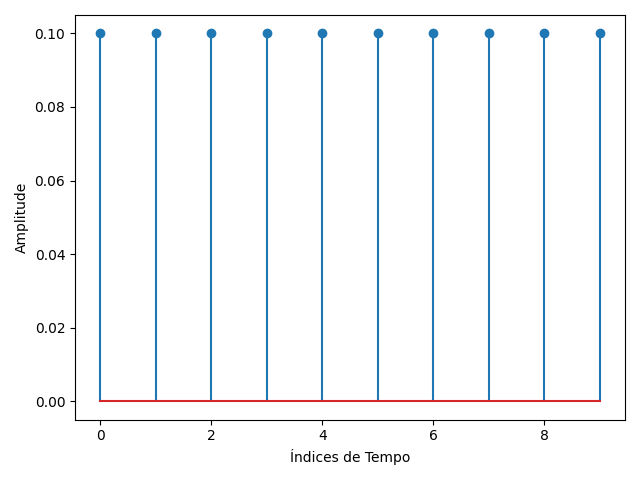
\includegraphics[width=\linewidth]{Imagens/fig21.png}
    \caption{Filtro h2[n] de média móvel com 10 amostras}
    \label{fig:graph_21}
\end{figure}

Na Figura \ref{fig:graph_22}, encontra-se o resultado da filtragem realziada pela média móvel de 10 amostras. A representação do resultado mostra uma senoide composta basicamente por uma frequência com pequenas distorções em amostras no início e ao final do período. Assim, esse item foi capaz de demonstrar a filtragem realizada por um simples filtro de média móvel.

\begin{figure}[!htb]
    \centering
    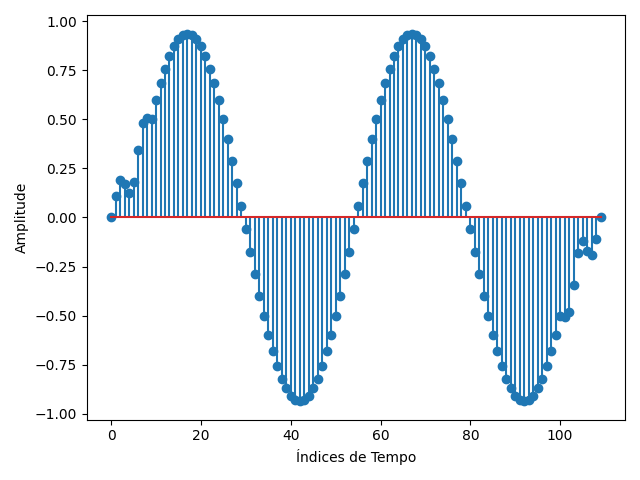
\includegraphics[width=\linewidth]{Imagens/fig22.png}
    \caption{Convolução de x[n] e h2[n]}
    \label{fig:graph_22}
\end{figure}

\newpage
\subsection{Item D}
Da mesma forma como se analisou a representação do processamento do sinal no domínio da frequência na questão dois, a mesma análise será realizada nesse item. Portanto, a análise do espectro do sinal original e do sinal filtrado será realizada e a filtragem poderá ser comprovada.

\begin{figure}[!htb]
    \centering
    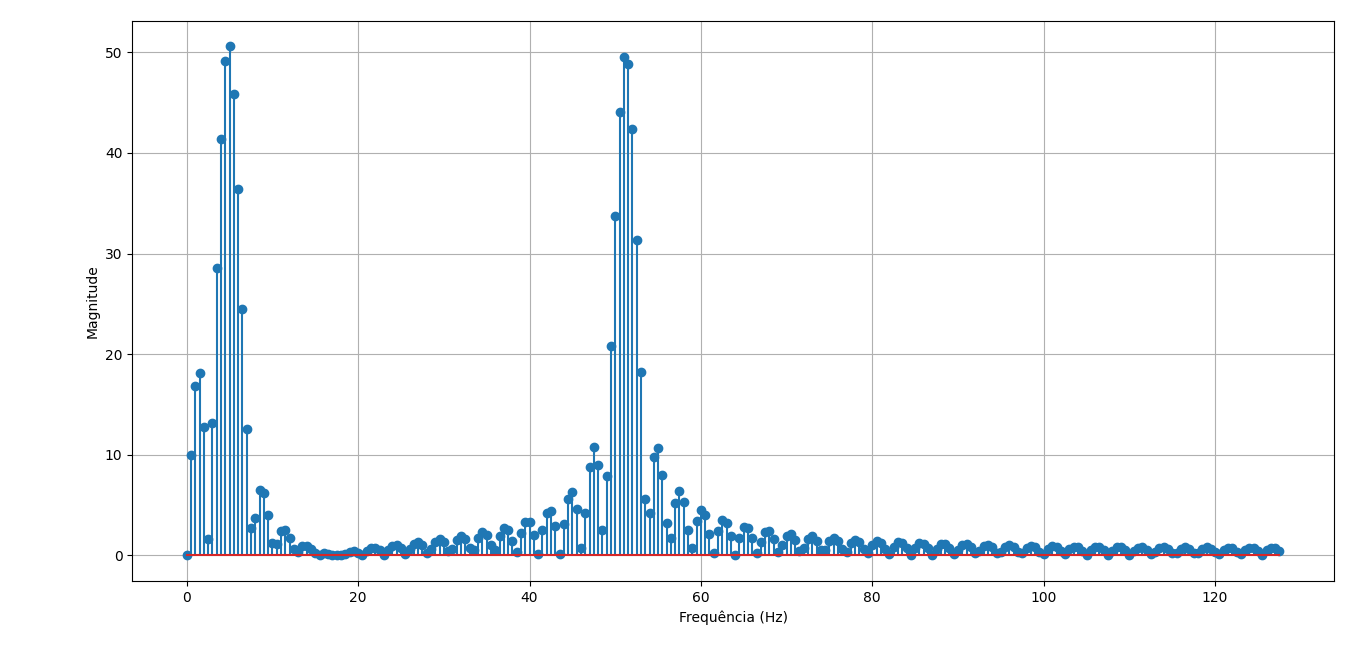
\includegraphics[width=\linewidth]{Imagens/fig23.png}
    \caption{Espectro em magnitude do sinal x[n]}
    \label{fig:graph_23}
\end{figure}

Na Figura \ref{fig:graph_23}, percebe-se as duas componentes de frequência que compõe o sinal $x[n]$. Uma componente está em uma baixa frequência e a outra está em uma frequência mais alta. 

Ao se utilizar o filtro de média móvel, a componente de alta frequência deve ser removida. Fato comprovado pela Figura \ref{fig:graph_24} na qual o espectro conta com apenas a componente em baixa frequência. 

\begin{figure}[!htb]
    \centering
    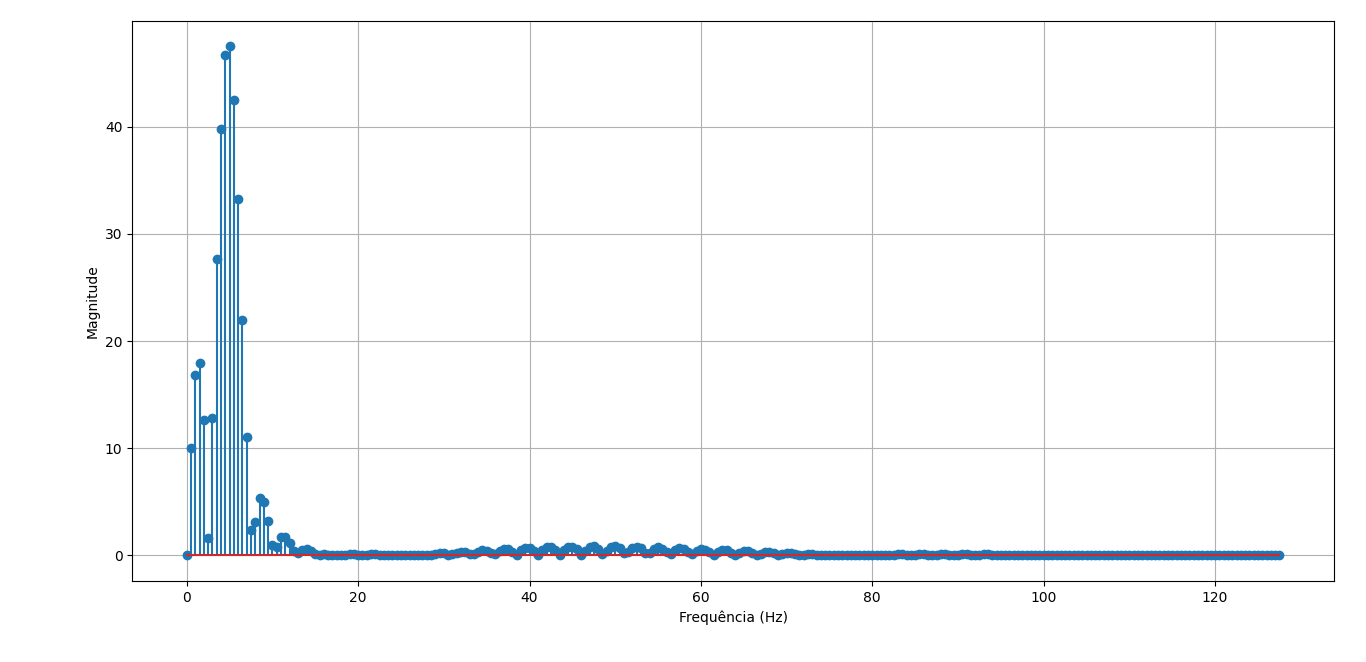
\includegraphics[width=\linewidth]{Imagens/fig24.png}
    \caption{Espectro em magnitude do sinal x[n] filtrado por média móvel}
    \label{fig:graph_24}
\end{figure}

A filtragem foi efetiva pois a constatação de que o sinal, após a filtragem, contém apenas a componente em baixa frequência pôde ser feita pelo sinal no domínio do tempo após a filtragem representada pela Figura \ref{fig:graph_22}.